\chapter{Evaluation}
\label{ch:evaluation}

This chapter details the evaluation process of the PIO device and SoC. Simulation was utilised as the primary verification technique, both through unit tests and testbenches, and through inspecting the output of example programs. Test software running on the SoC is also utilised.

FPGA Synthesis results are also presented, including utilisation and timing, and compared with current state of the art I/O hardware.

\section{Testbenches}

The primary tool used for verification is ChiselTest\footnote{\url{https://github.com/ucb-bar/chiseltest}}, introduced in Chapter \ref{ch:background}. For each module, unit test-style testbenches are written to verify that the hardware functioned as expected. ChiselTest uses Treadle\footnote{\url{https://github.com/chipsalliance/treadle}}, a high performance FIRRTL execution engine, as it's simulator backend by default. Treadle is used for simulation of the Chisel modules within the design, but does not include support for Verilog.

For modules written in Verilog, ChiselTest can still be used as the modules were wrapped as Chisel \txt{BlackBox} classes. ChiselTest can also target Verilator, a simulation tool that compiles Verilog to a high-performance cycle-accurate C++ model \cite{verilator}. Verilator has a longer startup time than Treadle due to the extra compilation steps involved, but is much faster, especially for larger designs. Verilator is used for the simulation of the full PIO device, as well as for unit testing of Verilog modules.


\begin{listing}[h!]
    \vspace{0.5cm}
    \begin{minted}{scala}
class ScratchRegTest extends AnyFlatSpec with 
  ChiselScalatestTester {
    "scratch register" should "read and write" in {
    test(new ScratchReg) { uut =>
    uut.io.write.data.poke(42)
    uut.io.write.enable.poke(true)
    uut.io.read.expect(0, "Clock not yet stepped, output should be 0")
    uut.clock.step()
    uut.io.read.expect(42, "Clock stepped, value 42 should be written")
    uut.io.write.data.poke(67)
    uut.clock.step()
    uut.io.read.expect(67, "Clock stepped with write enable still high, value 67 should be written")
    uut.io.write.enable.poke(false)
    uut.io.write.data.poke(78)
    uut.clock.step()
    uut.io.read.expect(67, "Clock stepped with write enable low, value 67 should remain")
    uut.clock.step(10)
    uut.io.read.expect(67, "Clock stepped with write enable low, value 67 should remain")
    }
    }
}
    \end{minted}
    \caption{An example test bench, used for testing the scratch register module.}
    \label{lst:test}
\end{listing}

An example unit test using ChiselTest is shown in Listing \ref{lst:test}. The primary method for verifying designs is by `poking' (setting) and `peeking' (reading) ports on the unit under test (\txt{uut}) while stepping the clock, and using \txt{expect} to make assertions about what the output should be. If the value in an \txt{expect} call does not match what the output, then the given error message, along with the failure of the location, is printed to assist with debugging. Waveform outputs of simulations can also be dumped to files for further inspection and debugging. An example test run for the scratch register test suite is show in Figure \ref{fig:testrun}, with both examples of passing and failing tests when invoked using sbt.

The codebase includes 52 unit unit tests, with at least one testbench for each module, which provides confidence in the correctness of the designs. Tests were mostly written before or alongside the modules themselves to enable a test-driven style of development, as discussed in Chapter \ref{ch:projman}.

\begin{figure}[H]
    \centering
    \subfloat[\centering Passing]{{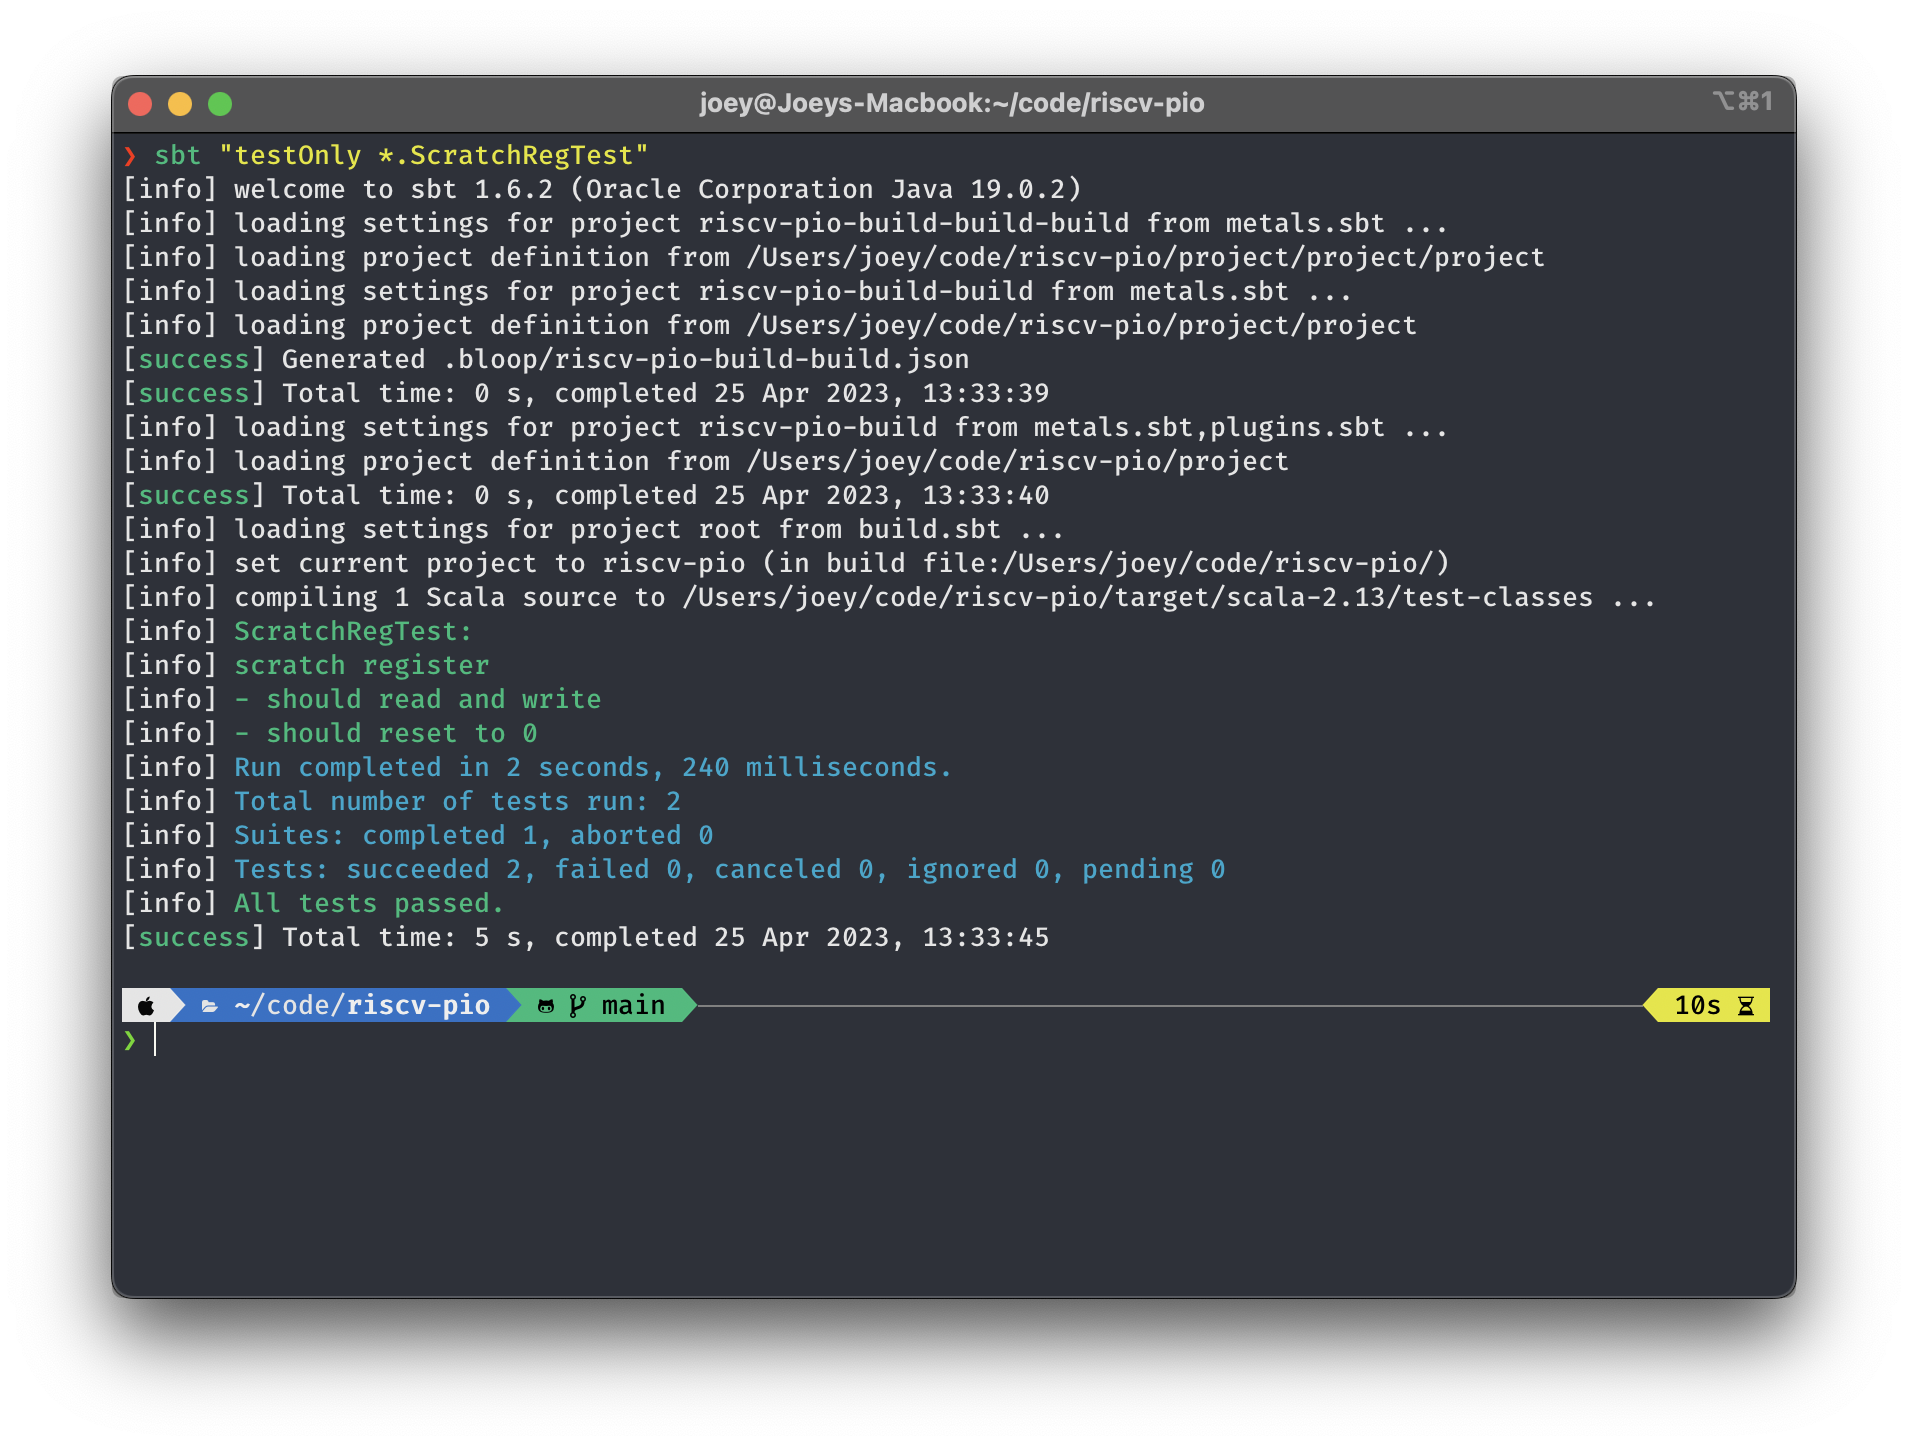
\includegraphics[width=0.45\textwidth]{../img/test-pass.png}} }
    \qquad
    \subfloat[\centering Failing]{{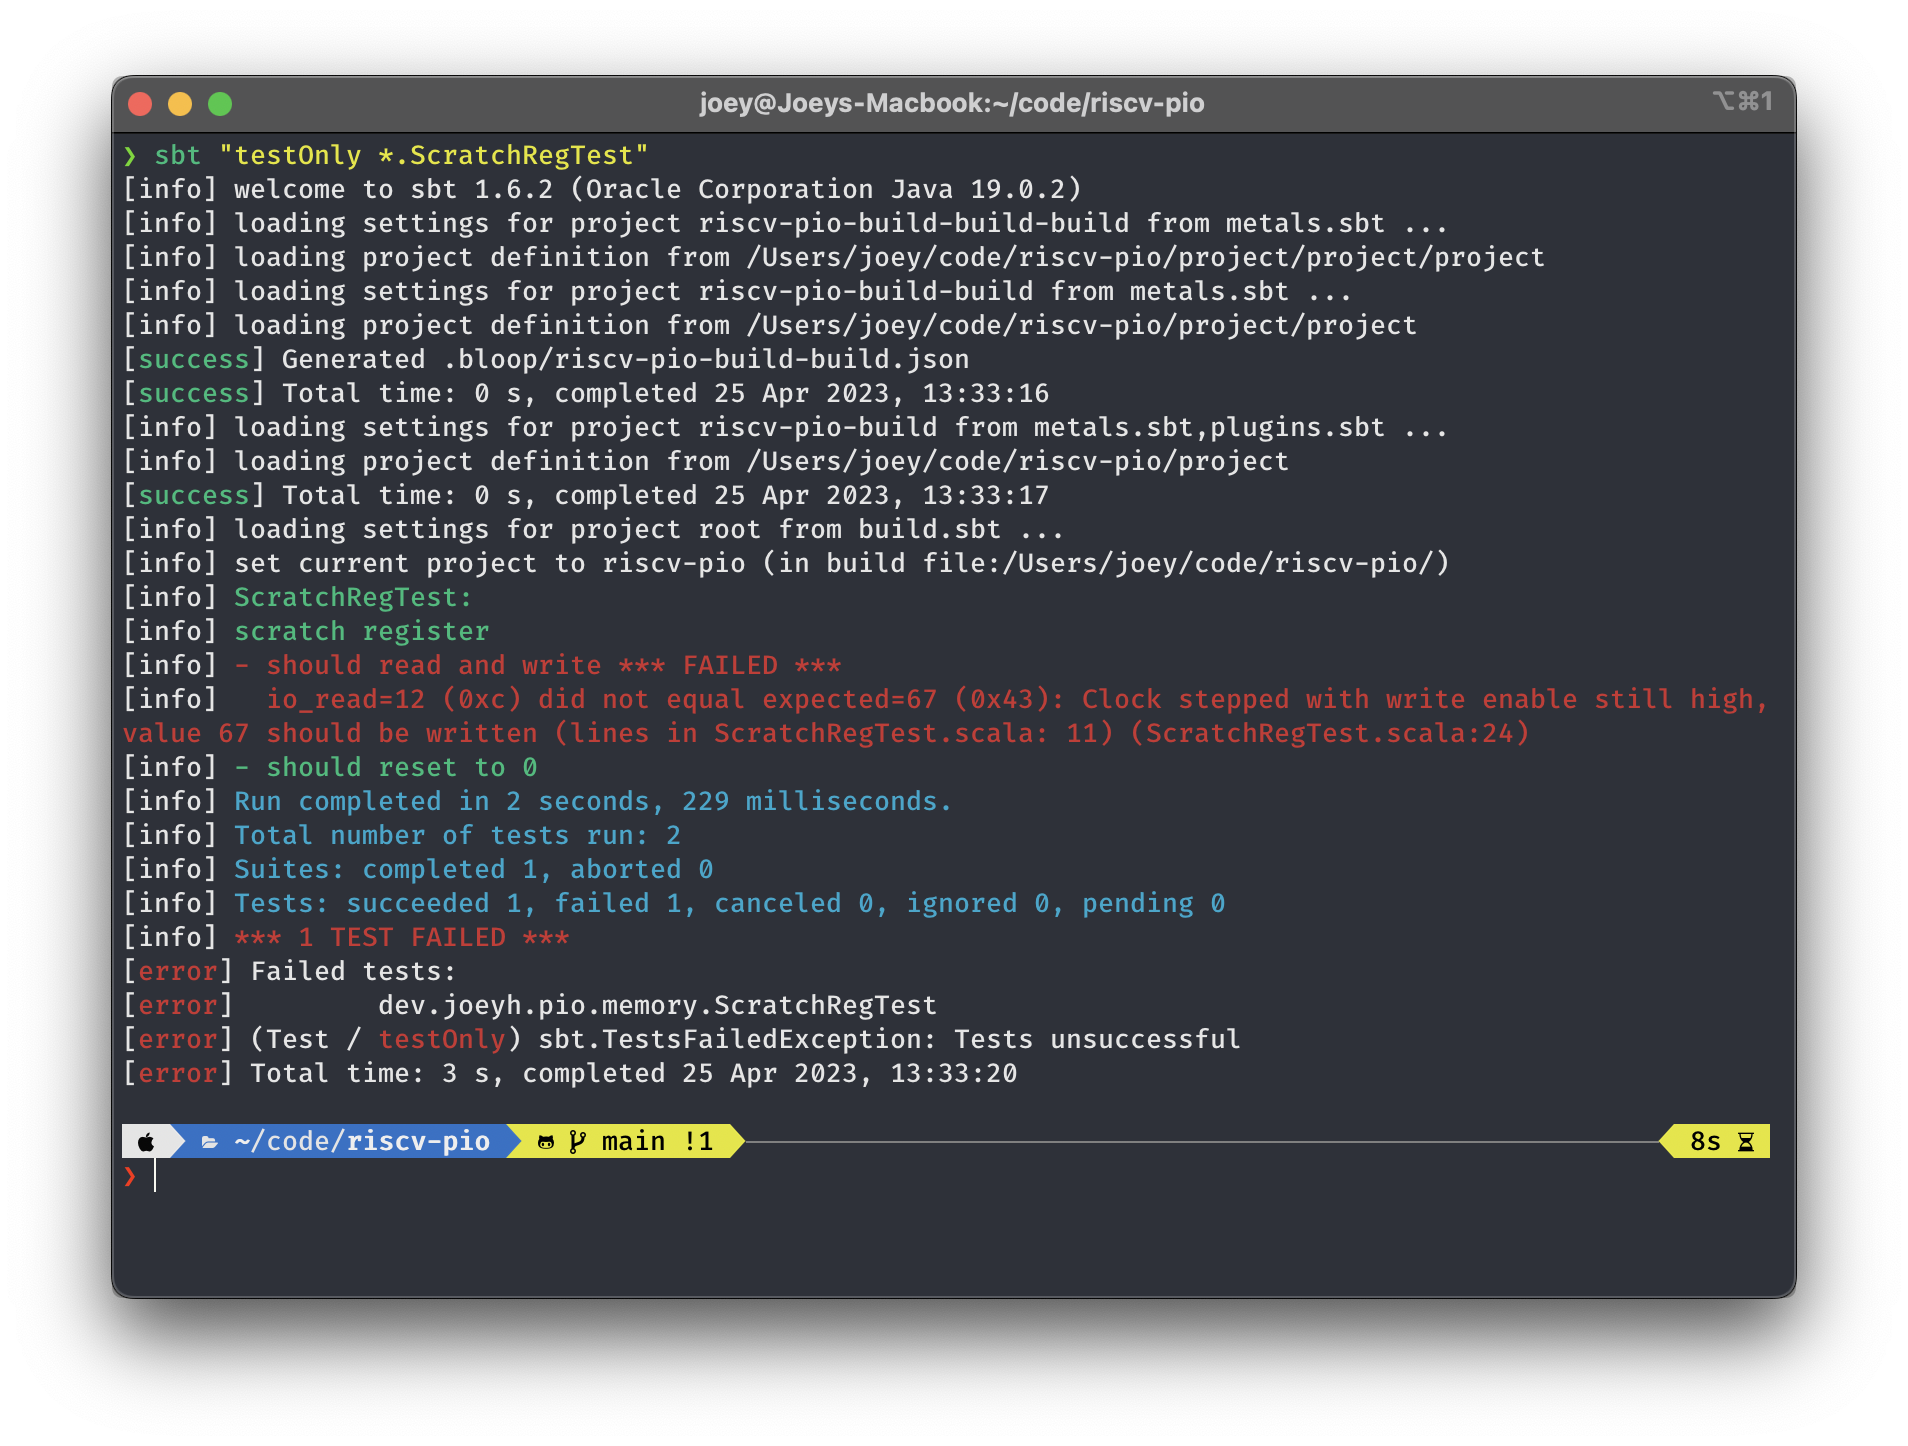
\includegraphics[width=0.45\textwidth]{../img/test-fail.png} }}
    \caption{Example outputs of test runs, invoked using sbt.}
    \label{fig:testrun}
\end{figure}


\section{Simulation \& Example Programs}
\label{sec:simulations}

A full simulation of the PIO block can be ran using a ChiselTest testbench for the top level PIO module, which then allows to interact with the PIO block the same as the SoC would. The memory port is used to write a program and set control registers, and then the clock is ran for a number of cycles. Instead of making assertions about the expected behaviour on a cycle-accurate level, the test waveforms are dumped to a file for manual inspection to verify that the system as a whole is functioning as expected. All internal signals can be inspected, allowing to verify the interactions between internal components as well as the correctness of the outward-facing behaviour.

\begin{listing}[h!]
    \begin{minted}{scala}
//an example program
val program = Seq(
    "b111_0_0001_110_00001".U,
    "b111_0_0000_110_00000".U, 
    "b000_0_0000_000_00000".U  
)
uut.io.rw.write.enable.poke(true)
//write each instruction
program.zip(Seq(0.U, 1.U, 2.U)).foreach {
case (a, i) =>
    uut.io.address.poke(i)
    uut.io.rw.write.data.poke(a)
    uut.clock.step()
}
    \end{minted}
    \caption{Sample code to write a program to PIO memory in simulation}
    \label{lst:sim-write-prog}
\end{listing}

Three example PIO programs are presented: a square wave, an SPI interface, and WS2812B serial.

\subsection{Square Wave}
\label{sec:blink-sim}

This is the most basic example, setting a pin high and then low in a loop to create a square wave that can be used to, for example, blink an LED.

\begin{listing}[h!]
    \begin{minted}{asm}
loop:
set pins, 1 [1]  //set output pin high, delay 1 cycle
set pins, 0      //set output pin low
JMP loop         //jump back to top
    \end{minted}
    \caption{RVPIO program to blink an LED}
    \label{lst:blinky}
\end{listing}

Very little configuration is required for this program. The clock divider is configured to give the desired frequency of the square wave, and the pin mapping is configured to have a single output pin and no inputs.

show waveform, explain

\subsection{WS2812B}

WS2812B LEDs are individually-addressable RGB LEDs that are usually connected in chains to create LED strips. They are addressable in such a way that the red, green, and blue colour component of each LED in a strip can be configured. When serial data is sent to an LED, it takes the first 3 bytes for it's own colour data and re-transmits the rest for the next LED in the chain \cite{picosdk,ws2812b}.

The LEDs have a very specific and non-standard serial pulse-width serial format. Each bit of data is transferred as a positive pulse, with the length of the pulse determing if the bit is high or low. Bit-banging this protocol is possible but hard due to the high speeds required, and emulating it over SPI introduces a lot of additional complexity. PIO is an ideal use case for these LEDs.

The RVPIO program to implement WS2812B serial is shown in Listing \ref{lst:ws2812b}.

\begin{listing}[h!]
    \begin{minted}{asm}

    \end{minted}
    \caption{RVPIO program to blink an LED}
    \label{lst:ws2812b}
\end{listing}

discuss config and timings

show waveform


\subsection{SPI}

SPI was first introduced by Motorola in 1979 in the same line of microcontrollers as the Motorola 86k designed for serial communication between digital electronics, and now ubiquitous within electronic components and peripherals. The interface is single-master multiple-slave using (at least) four signals: a clock, a master-out slave-in (MOSI) data line, master-in slave-out (MISO) data line, and a slave select (SS) line that is used for the master to signal when data is being transferred (one slave select line is used for each slave).

SPI can be implemented in 4 different modes, defined by the clock polarity (CPOL) and phase (CPHA) which determine which clock edges the data is toggled and sampled on. The most common, mode 0, toggles the MOSI line on the falling edge, and samples the MISO line on the rising edge, with the default clock state of low.

SPI can be implemented by PIO, the code for which is given in Listing \ref{lst:spi}. The example implements duplex SPI (shifting data in and out simultaneously) in mode 0. Slave select is not implemented by this example, as it's better suited to software GPIO control \cite{rp2040}.

\begin{listing}[h!]
    \begin{minted}{asm}
out pins, 1 side 0 [1] ; program stalls here on empty FIFO with clock low
in  pins, 1 side 1 [1] 
    \end{minted}
    \caption{RVPIO program to blink an LED \cite{rp2040}}
    \label{lst:spi}
\end{listing}

The program just shifts one bit at a time from the OSR out to the pins, and in from the pins to the ISR. The clock is controlled by the side-set. The program requires that autopull and autopush are both enabled such that data is automatically sent to/from the FIFOs. If the TX FIFO is empty, the program will stall with the clock low and no data will be sent or received. The pins mapping is configured to use a single input and a single output pin, which become the MISO and MOSI pins, with the clock being fixed to the side-set pin. The clock divider must also be configured at the correct speed for the peripheral.

results


\section{Test Software}

Test software is used to verify that the SoC as implemented on the FPGA functions correctly, and to demonstrate that the test programs work outside simulation, The software is written in Rust, and includes support for both the UART device to provide a serial console, and the PIO device.

The PIO device is modelled in software as shown in Listing \ref{lst:pio-rs}. We make use of the \txt{volatile_register}\footnote{\url{https://github.com/japaric/volatile-register}} library for abstracting over write-only device registers. The library provides the \txt{WO<T>} type with a single method, \txt{write(&mut self, value: T)} for performing a volatile write to the register. Volatile writes are needed to prevent certain optimisations\footnote{Rust has no formal memory model so the exact semantics of a volatile operation are not strictly defined. At the time of writing, the compiler is guaranteed not to relatively re-order or elide any volatile writes, and the semantics are similar to as defined by the C11 standard \cite{rust_pointer, c11}} by the compiler which may cause issues when working directly with hardware registers.

All of the registers are represented within a single struct, which when accessed through the correct pointer, provides access to the hardware pointers. Writing to raw pointers is an unsafe operation in Rust, and is only permitted by the compiler within explicitly marked \txt{unsafe} code blocks or functions. We make use of an unsafe function to construct the \txt{Pio} object, by casting the address which the registers are located at to the struct type, and then converting that to a static reference which is stored in a wrapper struct.

\begin{listing}[h!]
    \begin{minted}{rust}
const PIO_ADDR: usize = 0x6004_0000;
pub struct Pio(&'static mut PioRegisters);
#[repr(C)]
struct PioRegisters {
    instructions: [WO<u32>; 32],
    clock_div: WO<u32>,
    branch_pin: WO<u32>,
    wrap_config: WO<u32>,
    input_pin_config: WO<u32>,
    output_pin_config: WO<u32>,
    isr_config: WO<u32>,
    osr_config: WO<u32>,
    enable: WO<u32>,
}
impl Pio {
    pub unsafe fn new() -> Self {
        Pio((PIO_ADDR as *mut PioRegisters)
            .as_mut()
            .unwrap())
    }
    pub fn enable(&mut self) {
        unsafe { self.0.enable.write(1); }
    }
}
    \end{minted}
    \caption{Software model of the PIO hardware}
    \label{lst:pio-rs}
\end{listing}

The example program that we run is the square wave one, to blink an LED on the FPGA board. The code to run the program is not dissimilar to the simulation: write the same program and configuration as in Section \ref{sec:blink-sim} to the registers and then enable the PIO. The function is shown in Listing \ref{lst:blink-sw}. The function uses \txt{unsafe} blocks to perform register writes, as the compiler cannot guarantee that the write to the hardware is always valid.

\begin{listing}[h!]
    \begin{minted}{rust}
pub fn blink(pio: &mut Pio) {
    let program: [u32; 3] = [
        0b111_0_0001_110_00001,
        0b111_0_0000_110_00000,
        0b000_0_0000_000_00000,
    ];
    unsafe {
        for (a, i) in program.iter().enumerate() {
            pio.0.instructions[a].write(*i);
        }
        self.0.clock_div.write((u16::MAX - 1) as u32);
        self.0.output_pin_config.write(0x0100);
    }
    pio.enable();
}
    \end{minted}
    \caption{Rust function to initalise the PIO hardware with the square wave program in Listing \ref{lst:blinky}}
    \label{lst:blink-sw}
\end{listing}

The software is compiled to a static library using Cargo and Rustc, and then linked with some startup assembly code to call the main function using GCC. The linker also uses a linker script to lay out the binary in the correct way for the included bootloader to understand. The startup code, linker script and bootloader are provided by the same GitHub repository that provided the base SoC design.

The PIO input clock is 10MHz, so the clock divider is configured to be as slow as possible with a 16 bit clock divider (about 152Hz). FPGA synthesis constraints map PIO pins 0-15 to the board LEDs and pins 16-31 to the board switches, so the pin mapping is configured with PIO pin 0 as the single output pin.

The software and PIO both function as expected, blinking the configured LED on the FPGA board.

\section{Synthesis Results}
As discussed in Chapters \ref{ch:implementation} and \ref{ch:objectives}, an FPGA is used for implementation and the PIO block is synthesised as part of the SoC design. It is noted that the FPGA synthesis is used only for proof of concept, and that the proposed product fabricated as an ASIC, would have very different power and timing results.

\subsection{Utilisation}
\label{sec:synth-res}

FPGA utilisation results are given in Table \ref{tab:pio-util}. The design uses no block RAMs, as block RAMs are synchronous-read, requiring a cycle of delay to read values from. LUTs are used to implement asynchronous-read distributed LUTRAM instead for the instrution memory and control registers. No DSPs are used as there is not heavy arithmetic in the design, and the carry chains included in the regular logic slices are sufficient. The reason the logic and memory LUT utilisation do not sum to the total is that only approx 1/3 of LUTs can be used as LUTRAM. \cite{clb_ug}.

\begin{table}[h!]
    \centering
    \begin{tabular}{|c|c|c|}
        \hline
        \textbf{FPGA Element} & \textbf{Utilisation (No.)} & \textbf{Utilisation  (\%)} \\
        \hline
        \textbf{LUT (Logic)}  & 1482                       & 2.34\%                     \\
        \hline
        \textbf{LUT (Memory)} & 120                        & 0.63\%                     \\
        \hline
        \textbf{LUT (Total)}  & 1602                       & 2.53\%                     \\
        \hline
        \textbf{Register}     & 243                        & 0.19\%                     \\
        \hline
        \textbf{Block RAM}    & 0                          & 0\%                        \\
        \hline
        \textbf{DSP}          & 0                          & 0\%                        \\
        \hline
    \end{tabular}
    \caption{PIO utilisation results for the PIO block}
    \label{tab:pio-util}
\end{table}

The utilisation results for the entire SoC, including the Rocket core and other I/O components, is given in Table \ref{tab:soc-util}. The single-core design fits within the available FPGA resources comfortably. With optimisation of the Rocket core configuration, removing unnecessary components such as the MMU and FPU, it would be possible to generate a dual core SoC. The utilisation breakdown for the different SoC components is given in Figure \ref{fig:pie}.

\begin{table}[H]
    \centering
    \begin{tabular}{|c|c|c|}
        \hline
        \textbf{FPGA Element} & \textbf{Utilisation (No.)} & \textbf{Utilisation  (\%)} \\
        \hline
        \textbf{LUT (Logic)}  & 47016                      & 74.16\%                    \\
        \hline
        \textbf{LUT (Memory)} & 4151                       & 21.85\%                    \\
        \hline
        \textbf{LUT (Total)}  & 51167                      & 80.71\%                    \\
        \hline
        \textbf{Register}     & 31008                      & 24.45\%                    \\
        \hline
        \textbf{Block RAM}    & 15                         & 11.11\%                    \\
        \hline
        \textbf{DSP}          & 15                         & 6.25\%                     \\
        \hline
    \end{tabular}
    \caption{FPGA resource utilisation for the entire SoC design}
    \label{tab:soc-util}
\end{table}

\begin{figure}[H]
    \centering
    \begin{tikzpicture}
        \pie[text=legend, hide number]{58.18/Rocket core,
            8.96/DDR Memory Interface,
            5.85/I\/O AXI Interconnect,
            2.79/PIO,
            2.71/SD Card,
            1.29/Ethernet,
            1.24/Other,
            18.97/Unused}
    \end{tikzpicture}
    \caption{SoC LUT utilisation breakdown}
    \label{fig:pie}
\end{figure}

\subsection{Timing}

The design has no issues meeting timing constraints, despite the fact that the PIO is designed to execute all instructions within a single cycle. There is no negative slack in the entire design. The worst slack is 0.152ns in the SD card controller. The PIO used a 10MHz but there is plenty of slack in the design, indicating it could run at a much higher clock speed.

The path with the longest total delay within the PIO itself is one from the program counter to the ISR register, with a delay of 19.04ns, 16.99ns of which is interconnect delay. The rest of the other paths with the largest delay also were mostly interconnect delay. The large interconnect delay suggests that the place and route process took advantage of the loose timing constraints and placed the components further apart, increasing the clock speed may lead to more efficient routing.

The deepest logic paths within the PIO block are those implementing \txt{IN} and \txt{OUT} instructions: the control path from the program counter $\rightarrow$ instruction memory $\rightarrow$ instruction decoder $\rightarrow$ ISR logic $\rightarrow$ ISR register is the one with the most delay in the design, with a logic delay of 3.518ns. Similarly long delays are reported by paths that enable writes on scratch registers when shifting out from the OSR.

The deepest combinational paths \textit{through} the PIO block were those involved in reset signals. The reset for the AXI-Lite interface acts as the system reset for the PIO block, and is signalled by the Rocket core. The longest delay among these paths was 6.738ns, 93.2\% of which was interconnect delay, and still left a total slack of 12.83ns. This path originates in the Rocket core's 50MHz clock domain, hence the tighter timing constraint.

\subsection{Power}

The total on chip-power of the design is 1.158W, 109mW of which is static device power. Most of this power budget is accounted for by the interface with the external DDR memory (842 mW), as it runs at a much faster (200 MHz) clock speed than the rest of the design. The PIO device used only 2mW, slightly more than the 1mW used by the UART device, but much less than the 12mW used by the SD card controller.

maybe add another pie chart here, similar deal.

\section{Comparison with RP2040 \& existing hardware}

Comparing the RVPIO SoC to the RP2040 and it's PIO is difficult, as the RP2040 is a propietary piece of ASIC hardware for which no FPGA synthesis or timing results are available. However, in terms of functionality, the RVPIO is able to implement most of the same protocols as the RP2040 PIO as demonstrated in Section \ref{sec:simulations}. One major difference is that the a single RP2040 PIO block includes 4 state machines which can all execute independently, while the RVPIO is only can only execute a single program at a time, which limits the ability to implement more complex devices such as VGA controller and a USB sound card \footnote{\url{https://github.com/raspberrypi/pico-playground}}. The lack of DMA subsystem and system FIFO connections (discussed in Section \ref{sec:dma}) in the RVPIO SoC as currently implemented in the FPGA also prevents most useful applications from working outside of simulation.

The SoC as a whole is only a single core compared the the RP2040's two, and is much reduced in it's feature set as a microcontroller. However, the flexibility and customisability provided by both Rocket chip and RISC-V means this could be extended easily. This is enabled and encouraged by the open source nature of the RVPIO SoC, something which is a major advantage over the RP2040.

RVPIO is able to implement interfaces such as SPI and UART, but it's flexibility comes at a large cost compared to functionally equivalent fixed I/O blocks which typically use much fewer resources.

Anand et al. present a high-speed and compact SPI master and slave module in \cite{spi-device} that utilises only 50 LUTs and 47 flip flops as implemented in a Xilinx Virtex 5 FPGA: about 20x less than the RVPIO. A more featured SPI master is presented by Oudjida et al. in \cite{spi-i2c} that utilises 564 LUTs, implemented in the same FPGA architecture, indicating that more features and flexibility in the hardware comes at a cost of higher utilisation.

A UART device presented by Saha et al. in \cite{uart-device} utilises only 38 4-input LUTs and 28 flip flops, implemented in a Xilinx Spartan-2 FPGA, again indicating that fixed I/O hardware has the potential to be orders of magnitude more compact than RVPIO. The UART device included in the SoC template and implemented as part of the RVPIO SOC utilised XXX LUTs and YYY registers.

It is a trivial result that fixed function embedded I/O controllers use less FPGA resources than RVPIO. This is in contrast to Raspberry Pi's claim that RP2040 PIO state machines `are similar in size (and therefore cost) to a standard SPI peripheral' \cite{picosdk}. There are numerous reasons that their result may contradict ours: ASIC implementation details differ vastly from that of FPGAs, and the RP2040 PIO state machine architecture is likely much more compact. Their implementation is also far more optimised, something which is not true for our proof of concept.